% Chapter 1

\chapter{Software Implementation of the Inverter} % Main chapter title

\label{Chapter3} % For referencing the chapter elsewhere, use \ref{Chapter1} 

\lhead{Chapter 3. \emph{Software}} % This is for the header on each page - perhaps a shortened title

%----------------------------------------------------------------------------------------

\section{Software System Overview}
\label{softOver}
As with any microcontroller system, it is necessary to first configure the various low level peripherals such as the analog to digital converter (ADC), digital to analog converter (DAC), PWM, phase synchronization of PWM interrupts, PWM safety trips to avoid over-voltage conditions, clock and PLL configurations, and etc. The next step in the development was to design a logical, well organized and most importantly, extensible, software system to work with. The first phase in this development was to build a state framework for the organization of the various tasks associated with our power conversion system, namely the MPPT algorithm, tasks associated with power-up and shutdown, and instances where the power from the solar source is no longer sufficient to meet our output power guarantees. Quite secondarily, we also utilize these state machines to run LED indicators that show the code is operating as expected. The high level overview of the software can be seen in Figure \ref{soft}.

\begin{figure}[htp]
\begin{center}
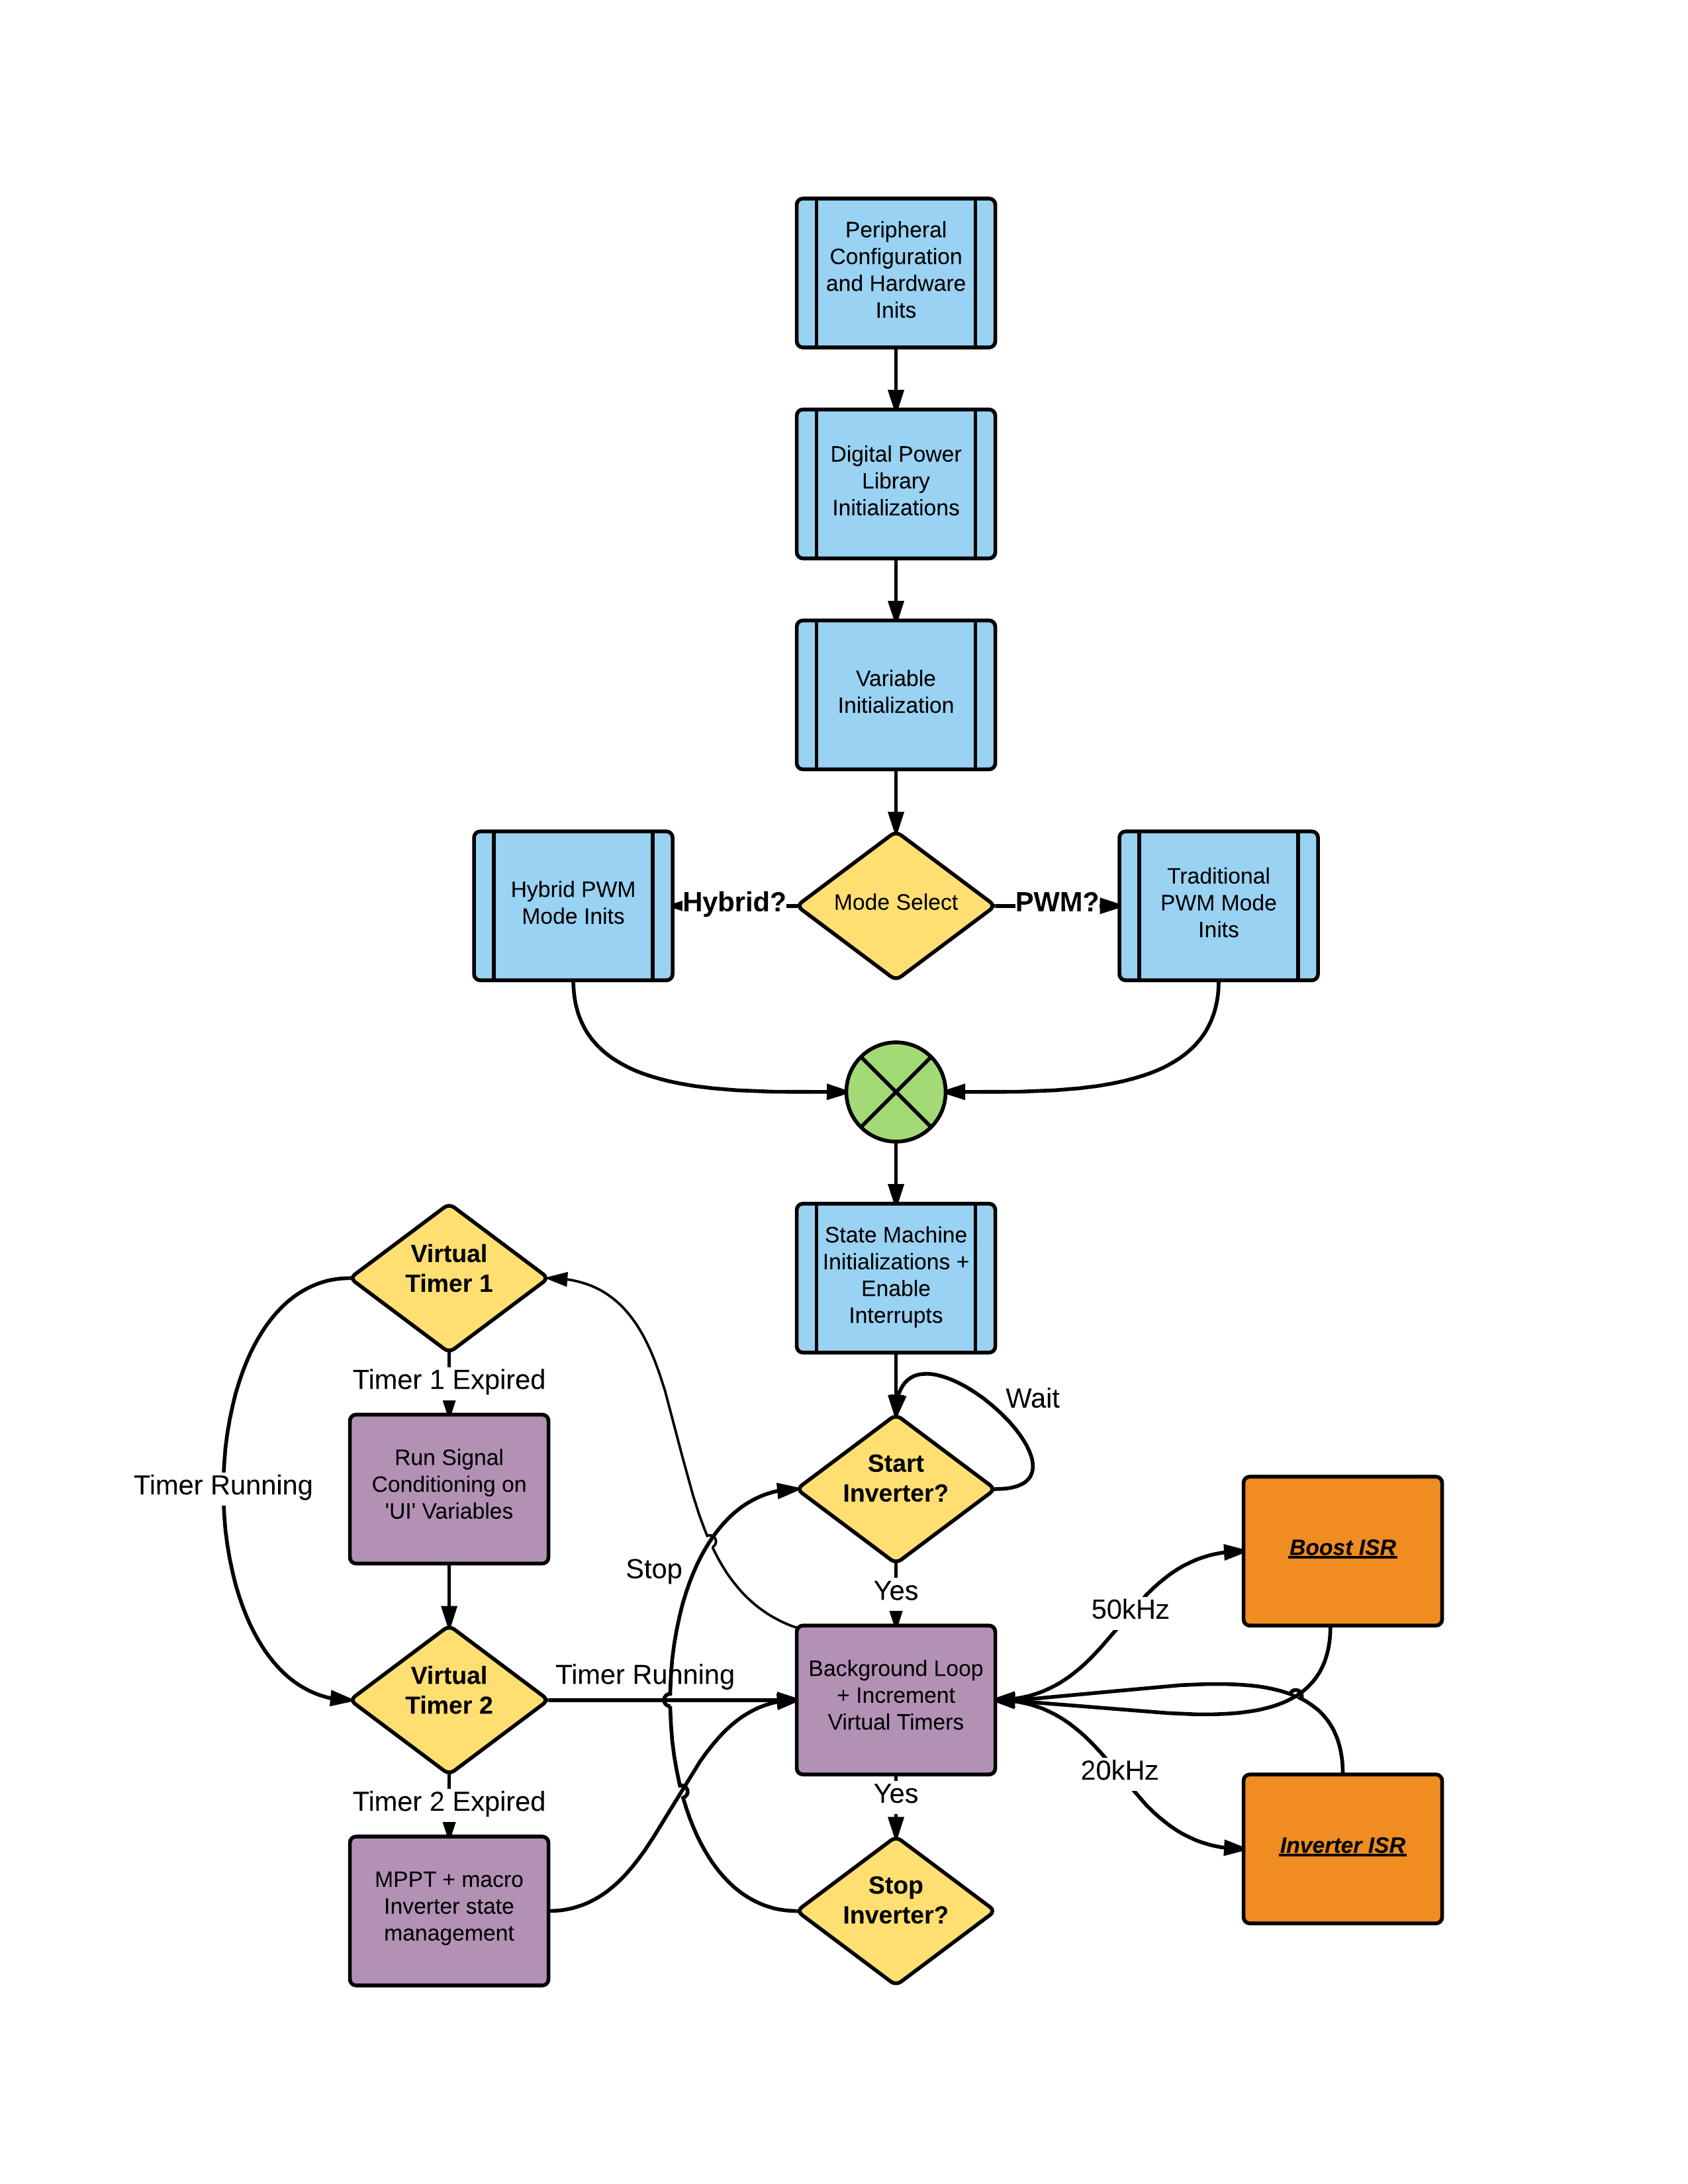
\includegraphics[height = \textheight, width = \textwidth, keepaspectratio]{softDiagramFinal}
\caption{Software system level overview showing the configuration of the micro, followed by an infinite loop where we run state machines on virtual timers, and service interrupts}
\label{soft}
\end{center}
\end{figure}

The two primary tasks of the software system are undoubtedly the control of the DC boost circuit, and the control of the inverter hardware. These tasks are pictured in Fig.\ref{fast} and Fig.\cite{slow} respectively. These tasks are performed using interrupt service routines (ISR)that are cued by the rising edge of a PWM signal. These signals offer a convenient way to trigger the interrupts, as well as the start of conversion (SOC) for the ADC. The SOC begins a sequential sampling of all the control signals on the board, making the most recent data available just in time for the execution of the ISR. Note that the PWM signals used for triggering interrupts are seperate from the PWM signals used for switching the transistors. With the execution of rapid-fire service routines, we may encounter the problematic condition where both ISRs attempt to fire at the same time. Instead of having the service routines fight for processor time with mechanisms like priorities, we opt to implement a phase synchronization scheme wherein the two PWM modules firing off interrupts are seperated by a pre-determined phase margin. This phase margin allows us to specify the time between rising edges of both PWM signals in relation to each other, the result being two dependent PWM channels that offer us an assurance that there will be no processor contention as long as we service either interrupt in a reasonable amount of clock cycles.

\begin{figure}[h]
\begin{center}
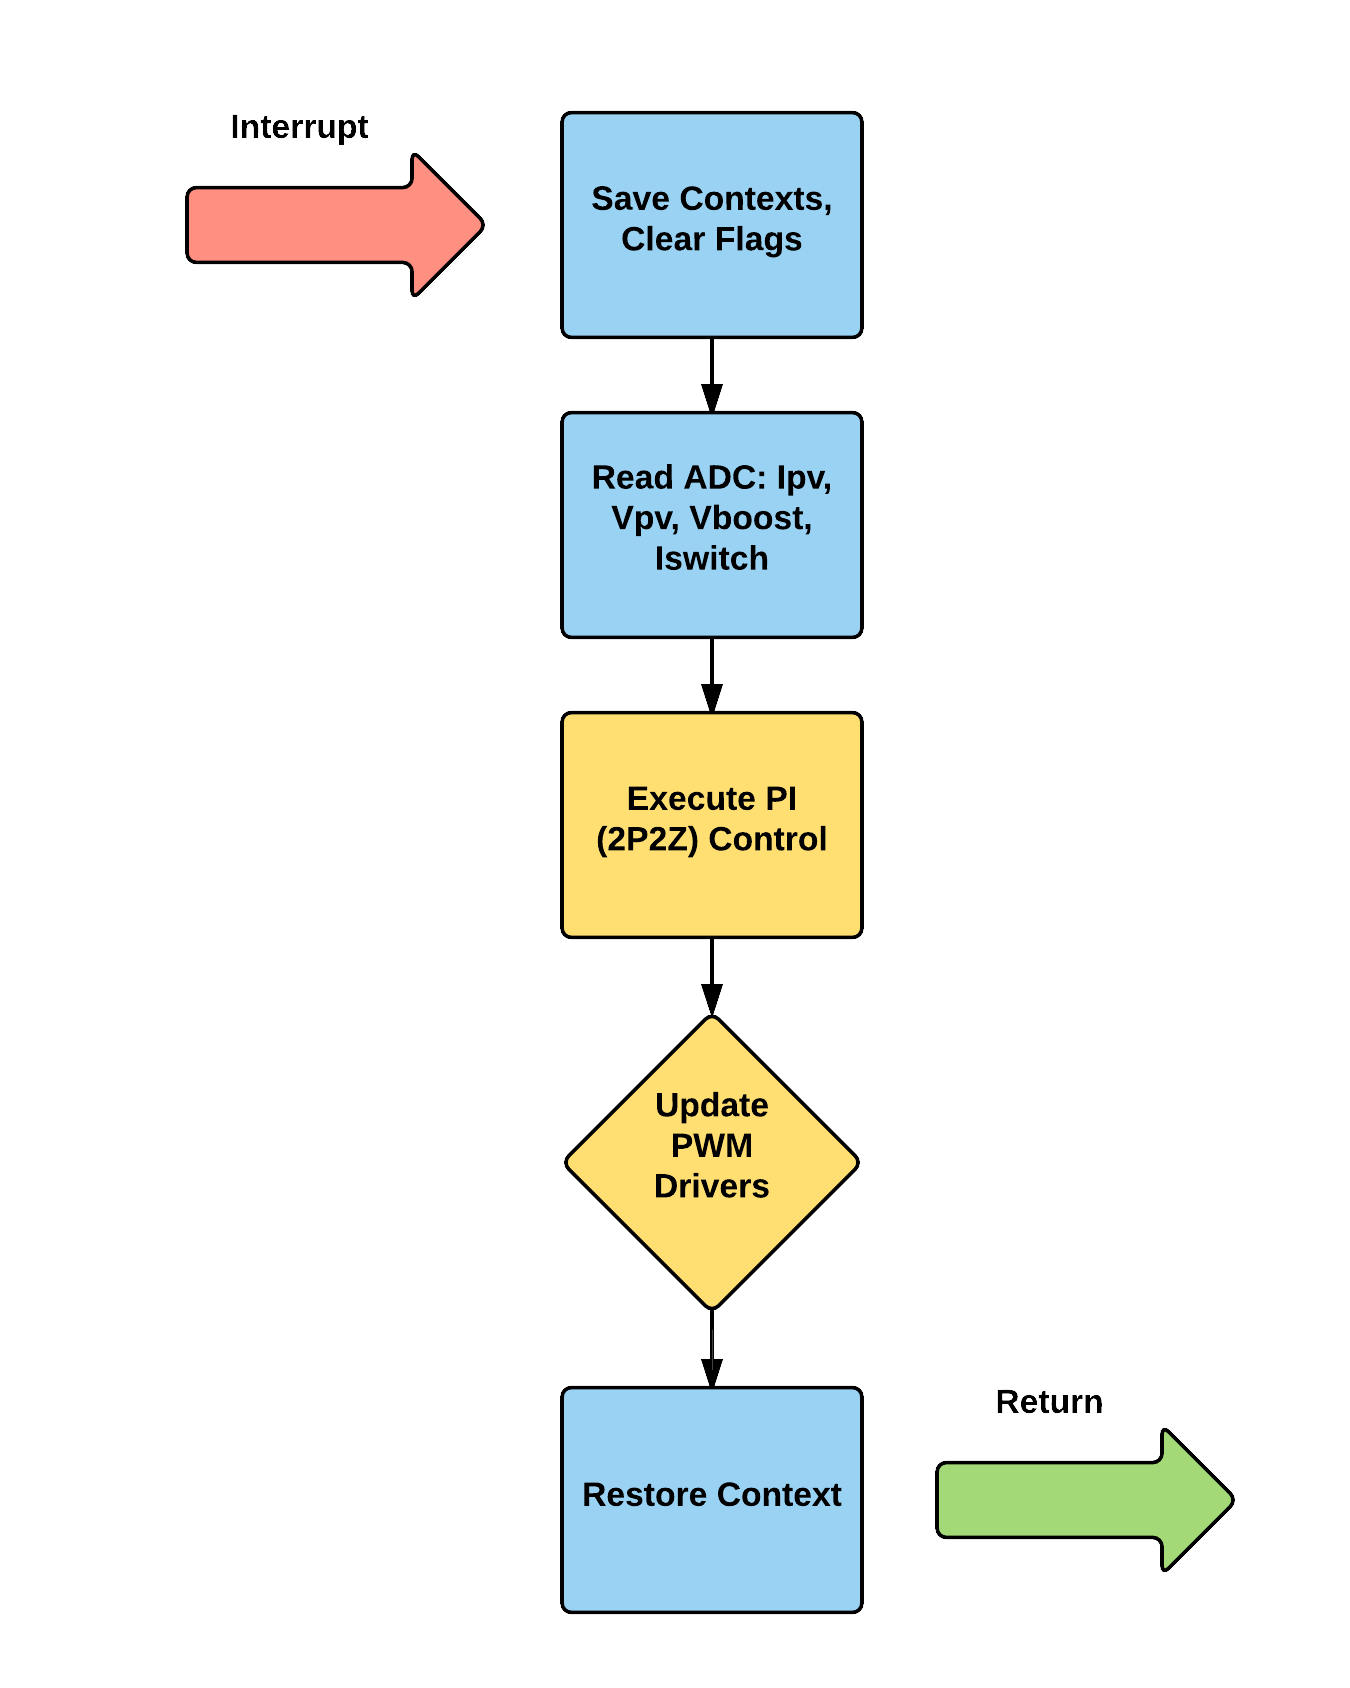
\includegraphics[width = 4 in]{boostISR}
\caption{Software diagram of the `fast' 50kHZ boost ISR}
\label{fast}
\end{center}
\end{figure}

\subsection{State Framework}
Although simple state frameworks are possible using functions as a sort of 'pseudo state,' these implementations tend to become exceedingly complex and hard to follow for non-trivial state machines. Further, cobbling together new state machines or adding new states can be a daunting task resulting in spaghetti code. 

For these reasons, we decided to 'roll our own' state framework using objected oriented patterns in C. This involved creating an FSM structure that holds a reference to an FSM object. This FSM object is actually a type defined variable that is, loosely speaking, of the type 'pointer to function'. Additionally, this strategy necessitated the implementation of several helper functions for various tasks like constructing the FSM object, state initialization, state transitions, and event dispatching. 

The custom 'pointer to function' type is declared in C as follows:
\begin{lstlisting}
typedef void (*State)(Fsm *, Event const *);
\end{lstlisting}

The definition above used the C keyword typedef. What typedef allows us to do is to declare a new data type for our own use. In this case, our type is 'pointer to function.' This is an enabling tool for representing the state of a machine as a function.

The next step trick is to use structures to organize all of our data in a meaningful way - for our purposes, you can think of these structs as classes, save for the fact that their methods are declared outside of the structure itself. Allow me to make a structure for the FSM itself, and call it 'Fsm.' Here's how we do it:

\begin{lstlisting}
struct Fsm
{      
        State state__; /* the current state */
};
\end{lstlisting}

The Fsm struct stores the function pointer as its sole attribute. Note that we use the trailing underscores to indicate that the variable is private and should not be tampered with in a nod to the Python style of adding leading underscores to indicate such members of classes. 

Students of electrical and computer engineering should be familiar with the concept that state machines respond to what are formally known as 'input alphabets.' These alphabets have strict definitions from a mathematical standpoint, but for our purposes, all we need to understand is that the machine should transition according to a certain mapping if it gets an event, and should - typically - do nothing if we do not send it an event. Accordingly, we should also declare some structure to manage event signals. This is done with

\begin{lstlisting}
struct Event
{
        Signal signal;
};
\end{lstlisting}

At this point we're ready to implement the functions that will manage this framework and allow for the creation of arbitrary state machines. These functions are inlined for speed - they eliminate a lot of the overhead of normal function calls - and they are well suited to this implementation since we are very concerned with speed and efficiency on our micros.

First up, we need to initialize the current state, i.e. give it something to point to. We will create an Fsm struct and invoke a function pointer for it to use. We will also set this pointer to the initial state of the FSM. We will do this with:

\begin{lstlisting}
#define _FsmCtor_(self_, init_) ((self_)->state__ = (State)(init_))
\end{lstlisting}

Next, it is desirable to go about triggering our initial transition. This is to say, our Fsm now points to the function we are using as the initialization state where we can do all the prep work we may need for the smooth operation of the Fsm, but now we want to get to work and make the machine run. We will trigger the initial transition with the following:

\begin{lstlisting}
#define FsmInit(self_, e_) (*(self_)->state__)((self_), (e_))
\end{lstlisting}

Now we've got a state machine that is in some state - the Fsm 'class' is pointing to some function we are using as a state - and we are ready to respond to events. How do we do it? With this inlined macro:

\begin{lstlisting}
#define FsmDispatch(self_, e_) (*(self_)->state__)((self_), (e_))
\end{lstlisting}


This will take some member of our particular Event structure that we defined above, and send the event to the function for it to respond to. This response is usually some action or state transition, or both.Finally, to round out our Fsm back-bone functions, we need something to actually implement the state transition, i.e. some function that updates the pointer and sets it to the new state when appropriate. This is accomplished with the following macro:
\begin{lstlisting}
#define _FsmTran_(self_, targ_) ((self_)->state__ = (State)(targ_))
\end{lstlisting}
Because the implementation of the state framework was, in our collective opinion, a major design hurdle, we feel it is productive to give the user a sense of the simplicity that this implementation imparts on FSM implementations. This is a particularly useful feature for us since we have several state machines in our systems, and the overall software design goal is extensibility.  

\begin{lstlisting}
int main()
{
    int returner = 0;
    hBridge k;
    hBridgeCtor(&k);
    FsmInit((Fsm *)&k, 0);
    for (;;)
    {
        hBridgeEvent ke;                   
        ke.code = getc(stdin); //replaced by ADC input in uC           
        getc(stdin);                      
        returner = hBridgeTransitionFunction(k, &ke);
        if(returner == -1) return 0;
        FsmDispatch((Fsm *)&k, (Event *)&ke);  //dispatch
    }
    return 0;
}
\end{lstlisting}
\hfill \break
\hfill \break
 
While this brief example departs from our actual implementation on the micro, it gives a quick overview of why the time spent developing this state framework was time well-spent, and hopefully provides some insight as to why the research into this area was worthwhile.

\subsection{The Digital Power Library}
One of the key features that made the Piccolo family of micro's an attractive option was the extensive power library that the the micro offered. In particular, the chip has the capability to run digital compensators of the 2P2Z form described in the section on the boost controller, and 3P3Z compensators as well. In addition, we have the ability to implement PID controllers with on-the-fly coefficient tuning via JTAG.

\section{The PWM Algorithm Implementation Details}
In order to assess the performance of the hybrid controller, we first needed to develop and assess the baseline performance of a typical PWM implemntation. This was done using the C2000 DSP which has generous functionality for accomplishing power conversion tasks. We decided to implement a unipolar PWM algorithm due to it's relative simplicity, and also because it is the most commonly implemented algortihm found on inverters today. The gist of the unipolar inverter algorithm is covered in Section \ref{pwmApproach}. Here, we will detail the specifics of the implemntation on the micro.

\begin{figure}[h]
\begin{center}
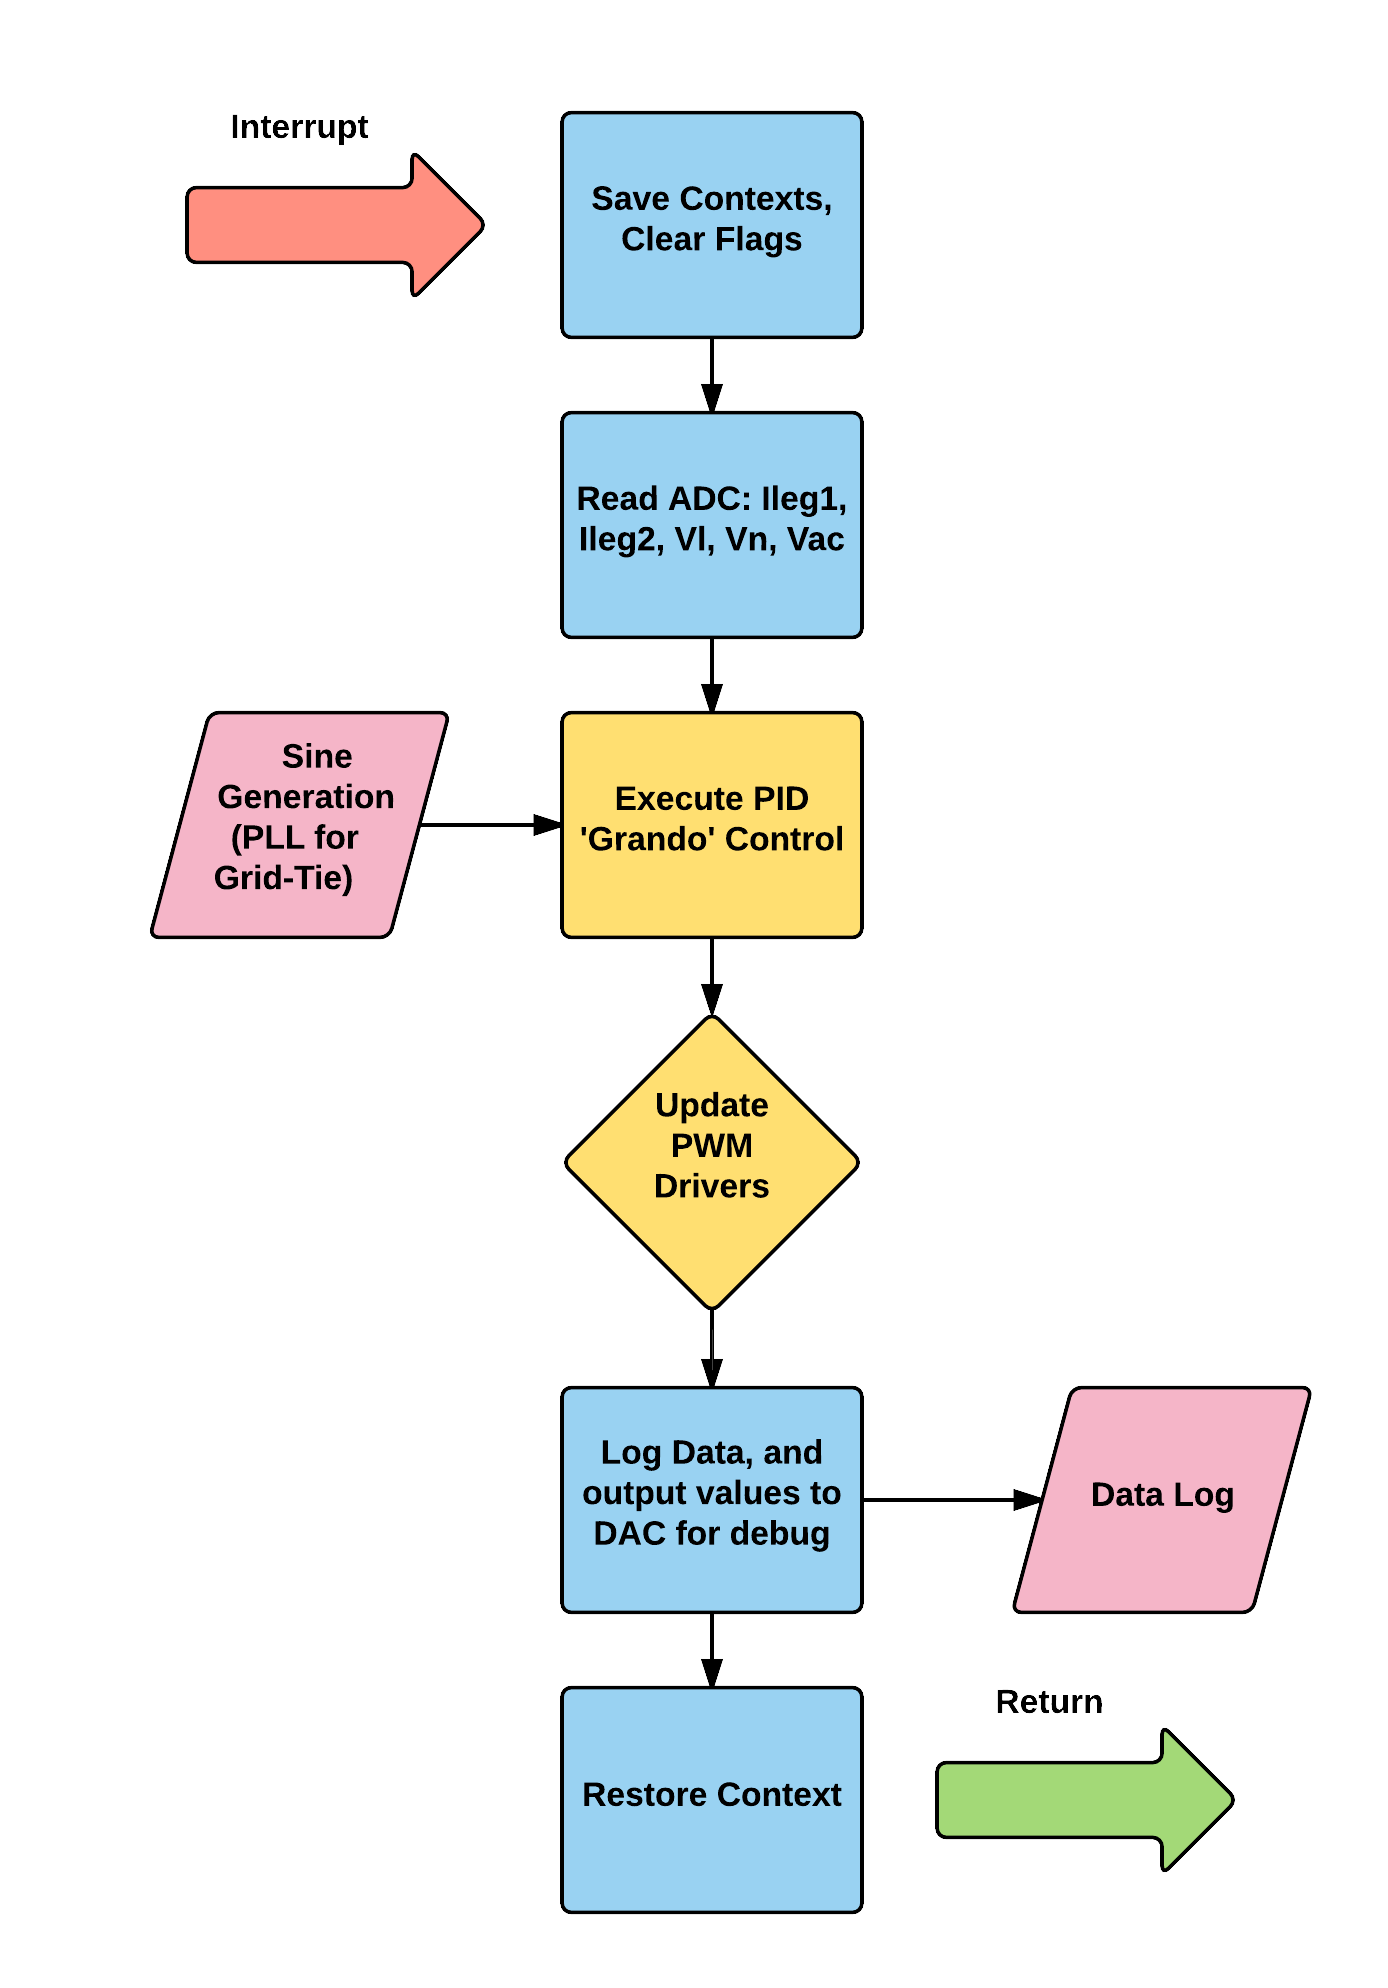
\includegraphics[width = 4 in]{traditionalISR}
\caption{Software diagram of the `slow' ~20kHZ traditional PWM inverter ISR}
\label{fast}
\end{center}
\end{figure}

Since the DC bus is not regulated by the boost stage feeding the inverter, the inverter itself uses nested control loops; the inner loop is for voltage control, and the outer loop employs current control. The voltage loop is used to provide a reference to the current loop; as the inverter is loaded and current demand increases, it is natural for the voltage to sag. The current reference at any instant is used with a software PID controller to provide the duty cycle to the inverter. To prevent current distortion, the voltage loop is only updated during zero-crossing events.

A unipolar inverter operates by comparing a triangular carrier wave to a sinusoidal reference signal. The triangular carrier wave generated is not a physical signal in our system, but rather an up-down counter set for a frequency of 20kHz in the case of the inverter's PWM. Using the Texas Instruments digital power library blocks, we then generate the sinusoidal reference. During the positive half cycle, if the sinusoidal reference becomes less than the triangular wave, the output of the PWM goes low. The resulting output waveform is sparse when the phase of the sinusoidal reference is near zero or $\pi$ radians, and becomes dense around $\frac{\pi}{2}$ radians. Inverse logic is true during the negative half-cycle. These comparisions are done by the PWM driver function, which is fed by the PID controllers of the inverter loop.

\section{Hybrid Algorithm Implementation Details}
In the initial stages of research and development, the hybrid inverter team first sought to recreate the simulations described in \cite{ricardo}. These simulations were best accomplished using the Hybrid Equations Toolbox in Matlab. Although the particulars of this implementation would be quite different than the final implementation in hardware, it was an excellent exercise in understanding the particulars of the algorithm, and also to give us a reference while implementing the hybrid controller on the C2000 micro controller in C. 

\subsection{The Matlab Implementation}
The first step in building the algorithm with Matlab was to translate the flow and jump sets into Matlab code. Determining which set the solution of the RLC filter is a member is critical in determining when to switch, and when to allow the differential equation solver to flow. 

These sets roughly translate as follows. Note that it can be helpful to refer to Figure \ref{jump} when deciphering the subsequent expressions. The flow set was translated as shown in \ref{lst:flowSetMatlab}.

The translation of the jump set is shown in the following code section. The jump set signals to the framework that it is time to change states. This requires that the solver change the set of equations that it is operating on. Determinning membership of the state variable in the jump set is done by the code given in \ref{lst:jumpSetMatlab}.

Now that we've determined whether we're in the flow set $C$, or the jump set $D$, we can perform the requisite logic for the controller. Here we give priority to jumps; this is to say, if we're in the sets $C$ and $D$, give priority to the jump set and perform the necessary state transition instead of continuing to flow continuously. If we're in the jump set, this signals to the controller that we ought to execute a transition according to the jump map given in \ref{lst:jumpMapMatlab}.

In the code, 'qplus' refers to the state that we're going to jump to, and 'pplus' refers to a change of controller. For example, if $q$ is equal to zero, and 'qplus' is found to be one, then the next state of the H-Bridge will be to output $+V_{DC}$. Likewise, if the current controller variable $p$ is equal to two - indicating that the global controller is in the loop - and 'pplus' is found to be one, then the forward controller will take over on the next update. 

This is the bulk of the code for the Matlab simulations, though we have omitted the description of the behavior of the system as the solution flows, as this is covered in detail in \cite{ricardo}.

\subsection{The C Implementation on the C2000}
We aim to briefly clarify the mechanisms behind how the hybrid inverter works, and discuss the process we undertook in implementing the hybrid algorithm on our custom hardware validation platform. 

\begin{figure}[h]
\begin{center}
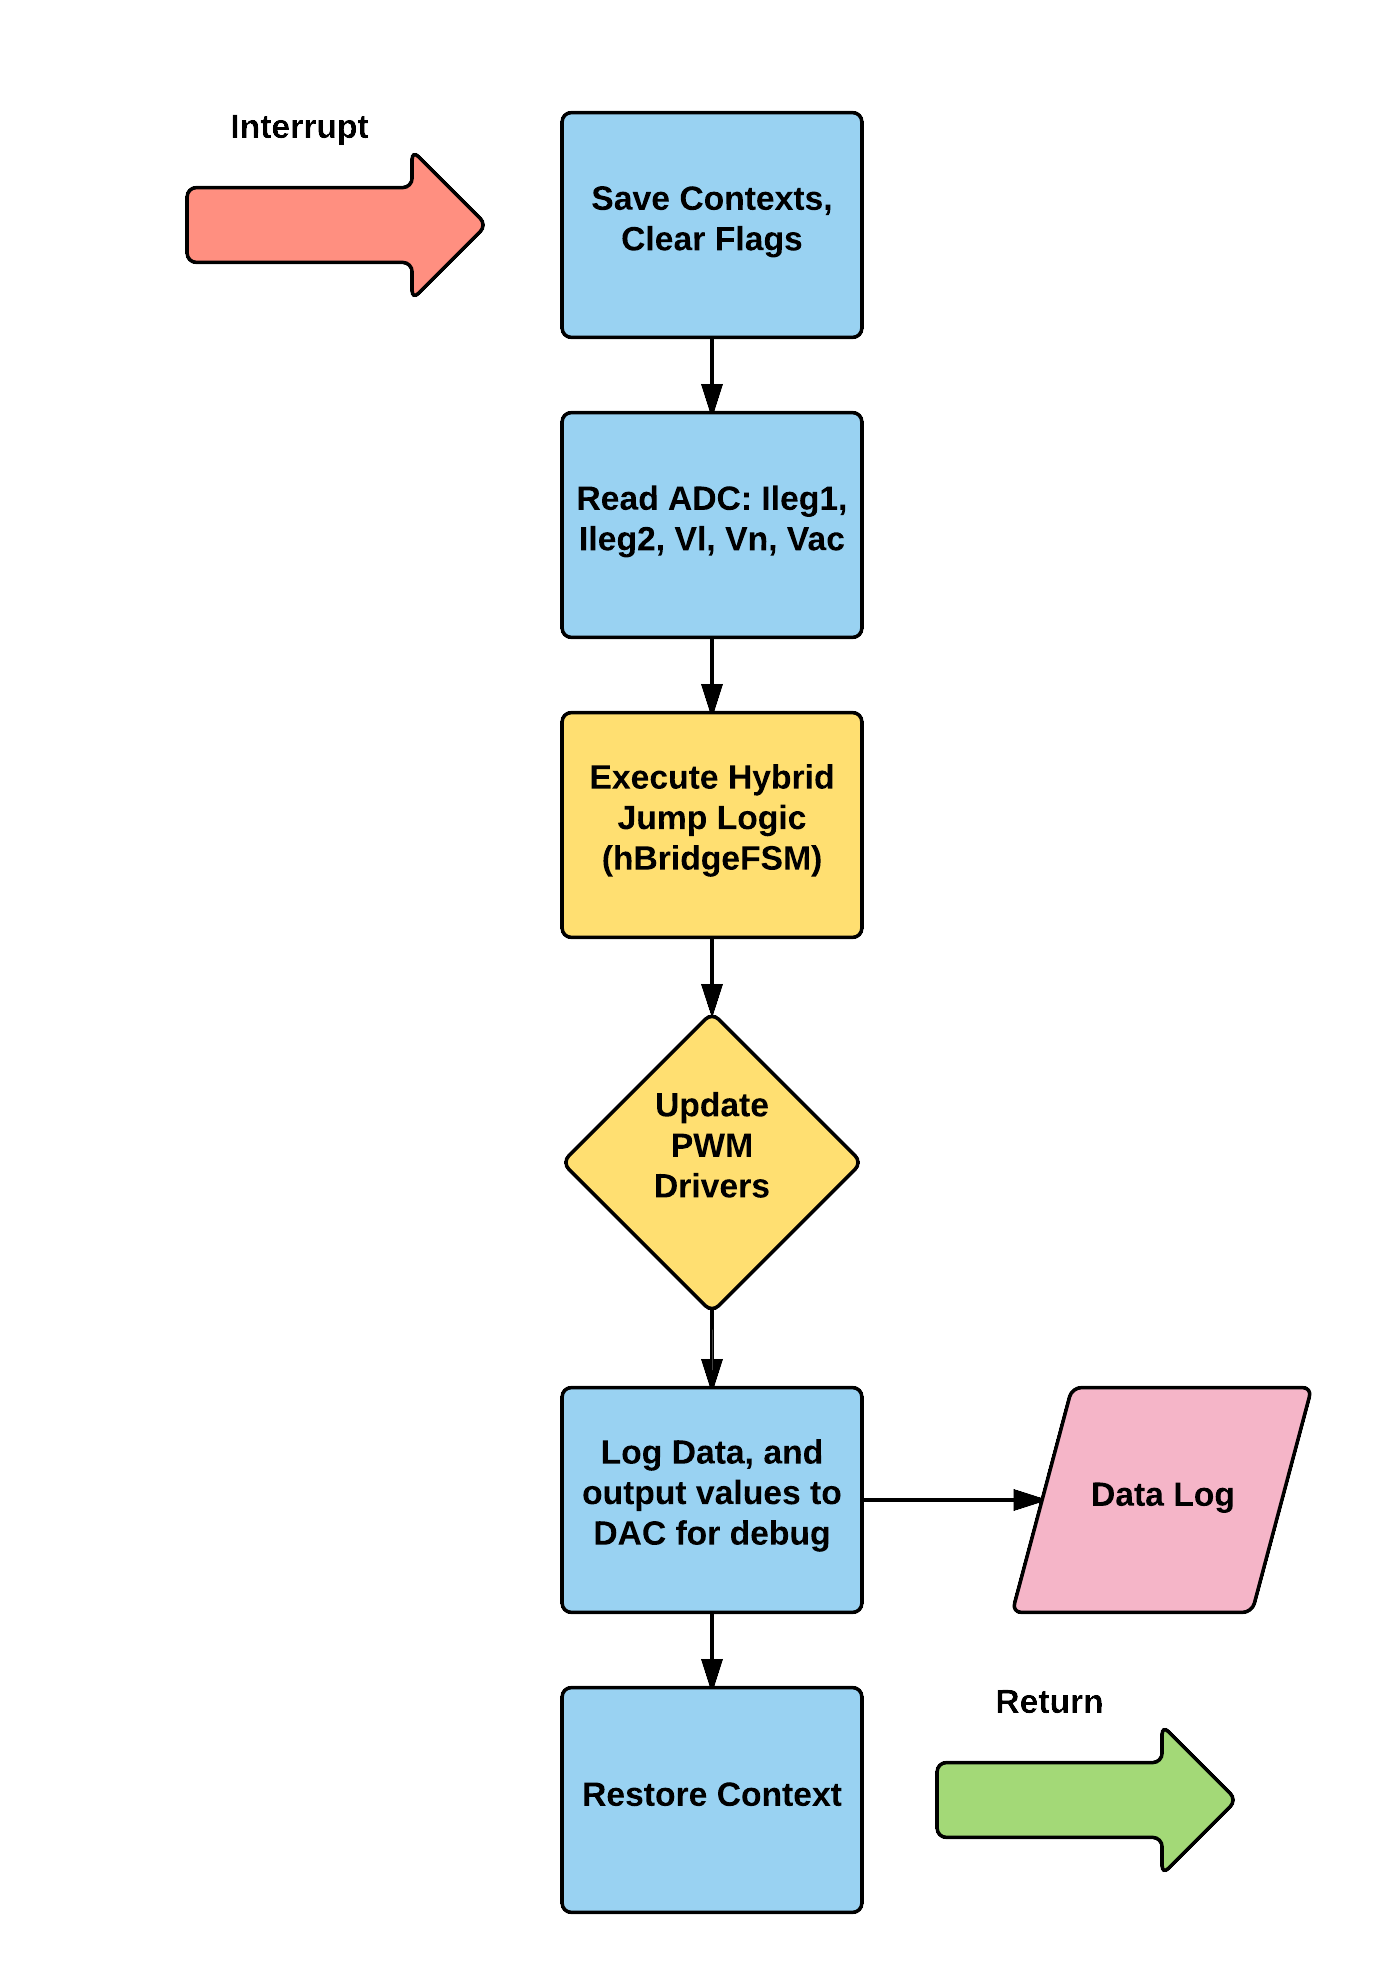
\includegraphics[width = 4 in]{hybridISR}
\caption{Software diagram of the `slow' ~20kHZ hybrid PWM inverter ISR}
\label{fast}
\end{center}
\end{figure}

The derivation of the hybrid control algorithm is roughly as follows: given that the response of a series RLC filter can be thought of as a linear oscillator with a damping term, and given that we have a set of desired output parameters - namely the amplitude of the output voltage, the amplitude of the output current, and the angular frequency $\omega$, then by solving the resultant linear differential equation, we can derive a reference solution for the given system to a perfect sinusoidal driving signal. In reality we will not have a sinusoidal driver, but rather some permutation of a square wave capable of switching between $+V_{dc}$, $-V_{dc}$ and $0$, where $V_{dc}$ is the DC bus voltage at the input to the H-Bridge controlled by the state variable $q$. We consider $q=1$ to correspond to $+V_{dc}$, $q=-1$ to correspond to $-V_{dc}$, and $q=0$ to correspond to $0$. This process is illustrated clearly in Figure \ref{jumpMap}.

\begin{figure}[htbp]
\begin{center}
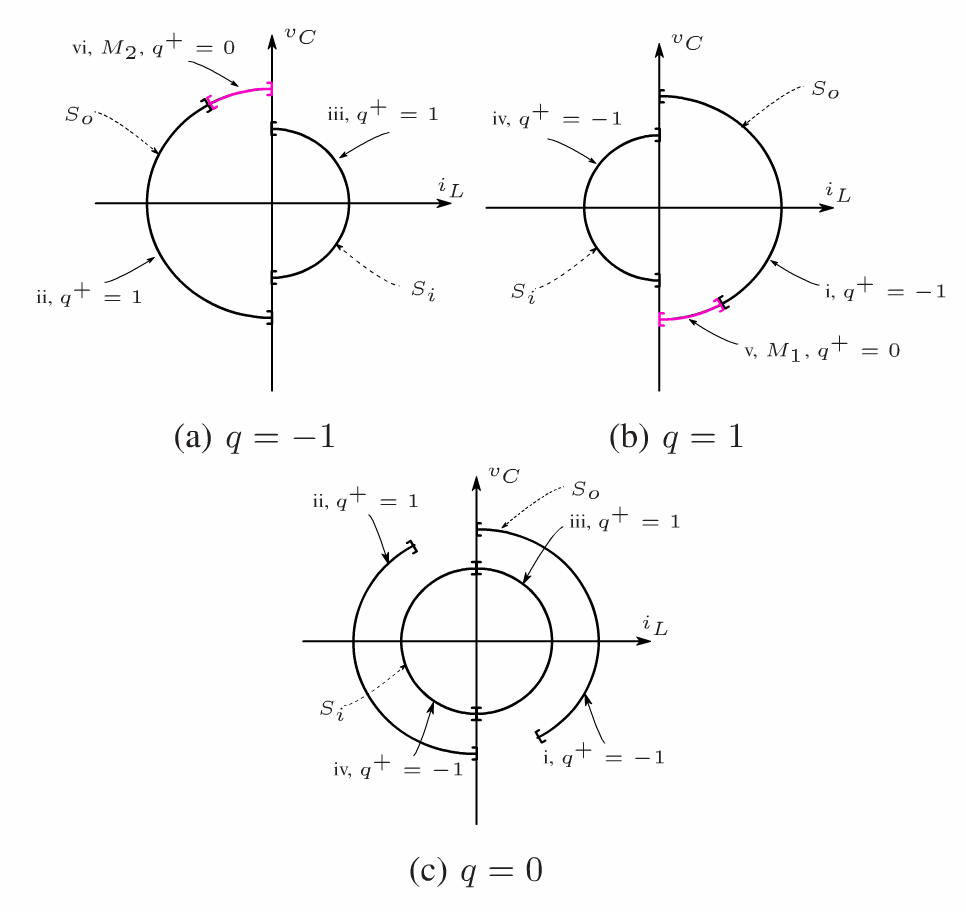
\includegraphics[width = 3.5 in]{jumpMap}
\caption{Jump Map of the Hybrid Algorithm \cite{ricardo}}
\label{jump}
\end{center}
\end{figure}

We can think of the resultant solution to the sinusoidal driver as the ideal to which our system should strive, and therefore any deviation from this ideal can be considered as an error that needs to be corrected by the controller. These errors are detected by building a tracking band around the reference solution; this is done by choosing a neighborhood around the reference solution. Collectively, this region is known as the tracking band. Now, if we consider the instantaneous state of the system to be a vector made up of the capacitor voltage and the current through the inductor, then we can measure the location of the vector in relation to the tracking band on the VI plane. Since the inductor and capacitor are at all times 90 degrees out of phase without any load or perturbation, the ideal solution takes the shape of an ellipse on the VI plane. By taking the state vector's position relative to the tracking band, and knowing the trajectory at a given region on the VI plane, it is straightforward to develop a small set of rules governing the switching of the inverter, i.e. the jump between the three states of the H-bridge circuit, namely $q=1$, $q=-1$, and $q=0$. With this brief foundation, we are able to steer the state of the system around the VI plane, with the resultant output being a pseudo-sinusoid with the desired voltage and current amplitude and frequency. 

With the logic for the controller worked out in Matlab, the work of porting the code to embedded C on the Texas Instruments DSP was a matter of fitting this logic within the bounds of the hardware modules onboard.
In the sections above, namely Section \ref{softOver}, we discussed that the general flow of the software on the C2000 DSP is to first initialize and configure the hardware modules onboard, then to service interrupts for the boost converter and the inverter. Of chief concern in this section is the inverter ISR where we call upon a state machine that determines membership in the jump set, then informs the hardware of the appropriate action to take. The state machine is implemented using the custom state framework described above.

\begin{figure}[h]
\begin{center}
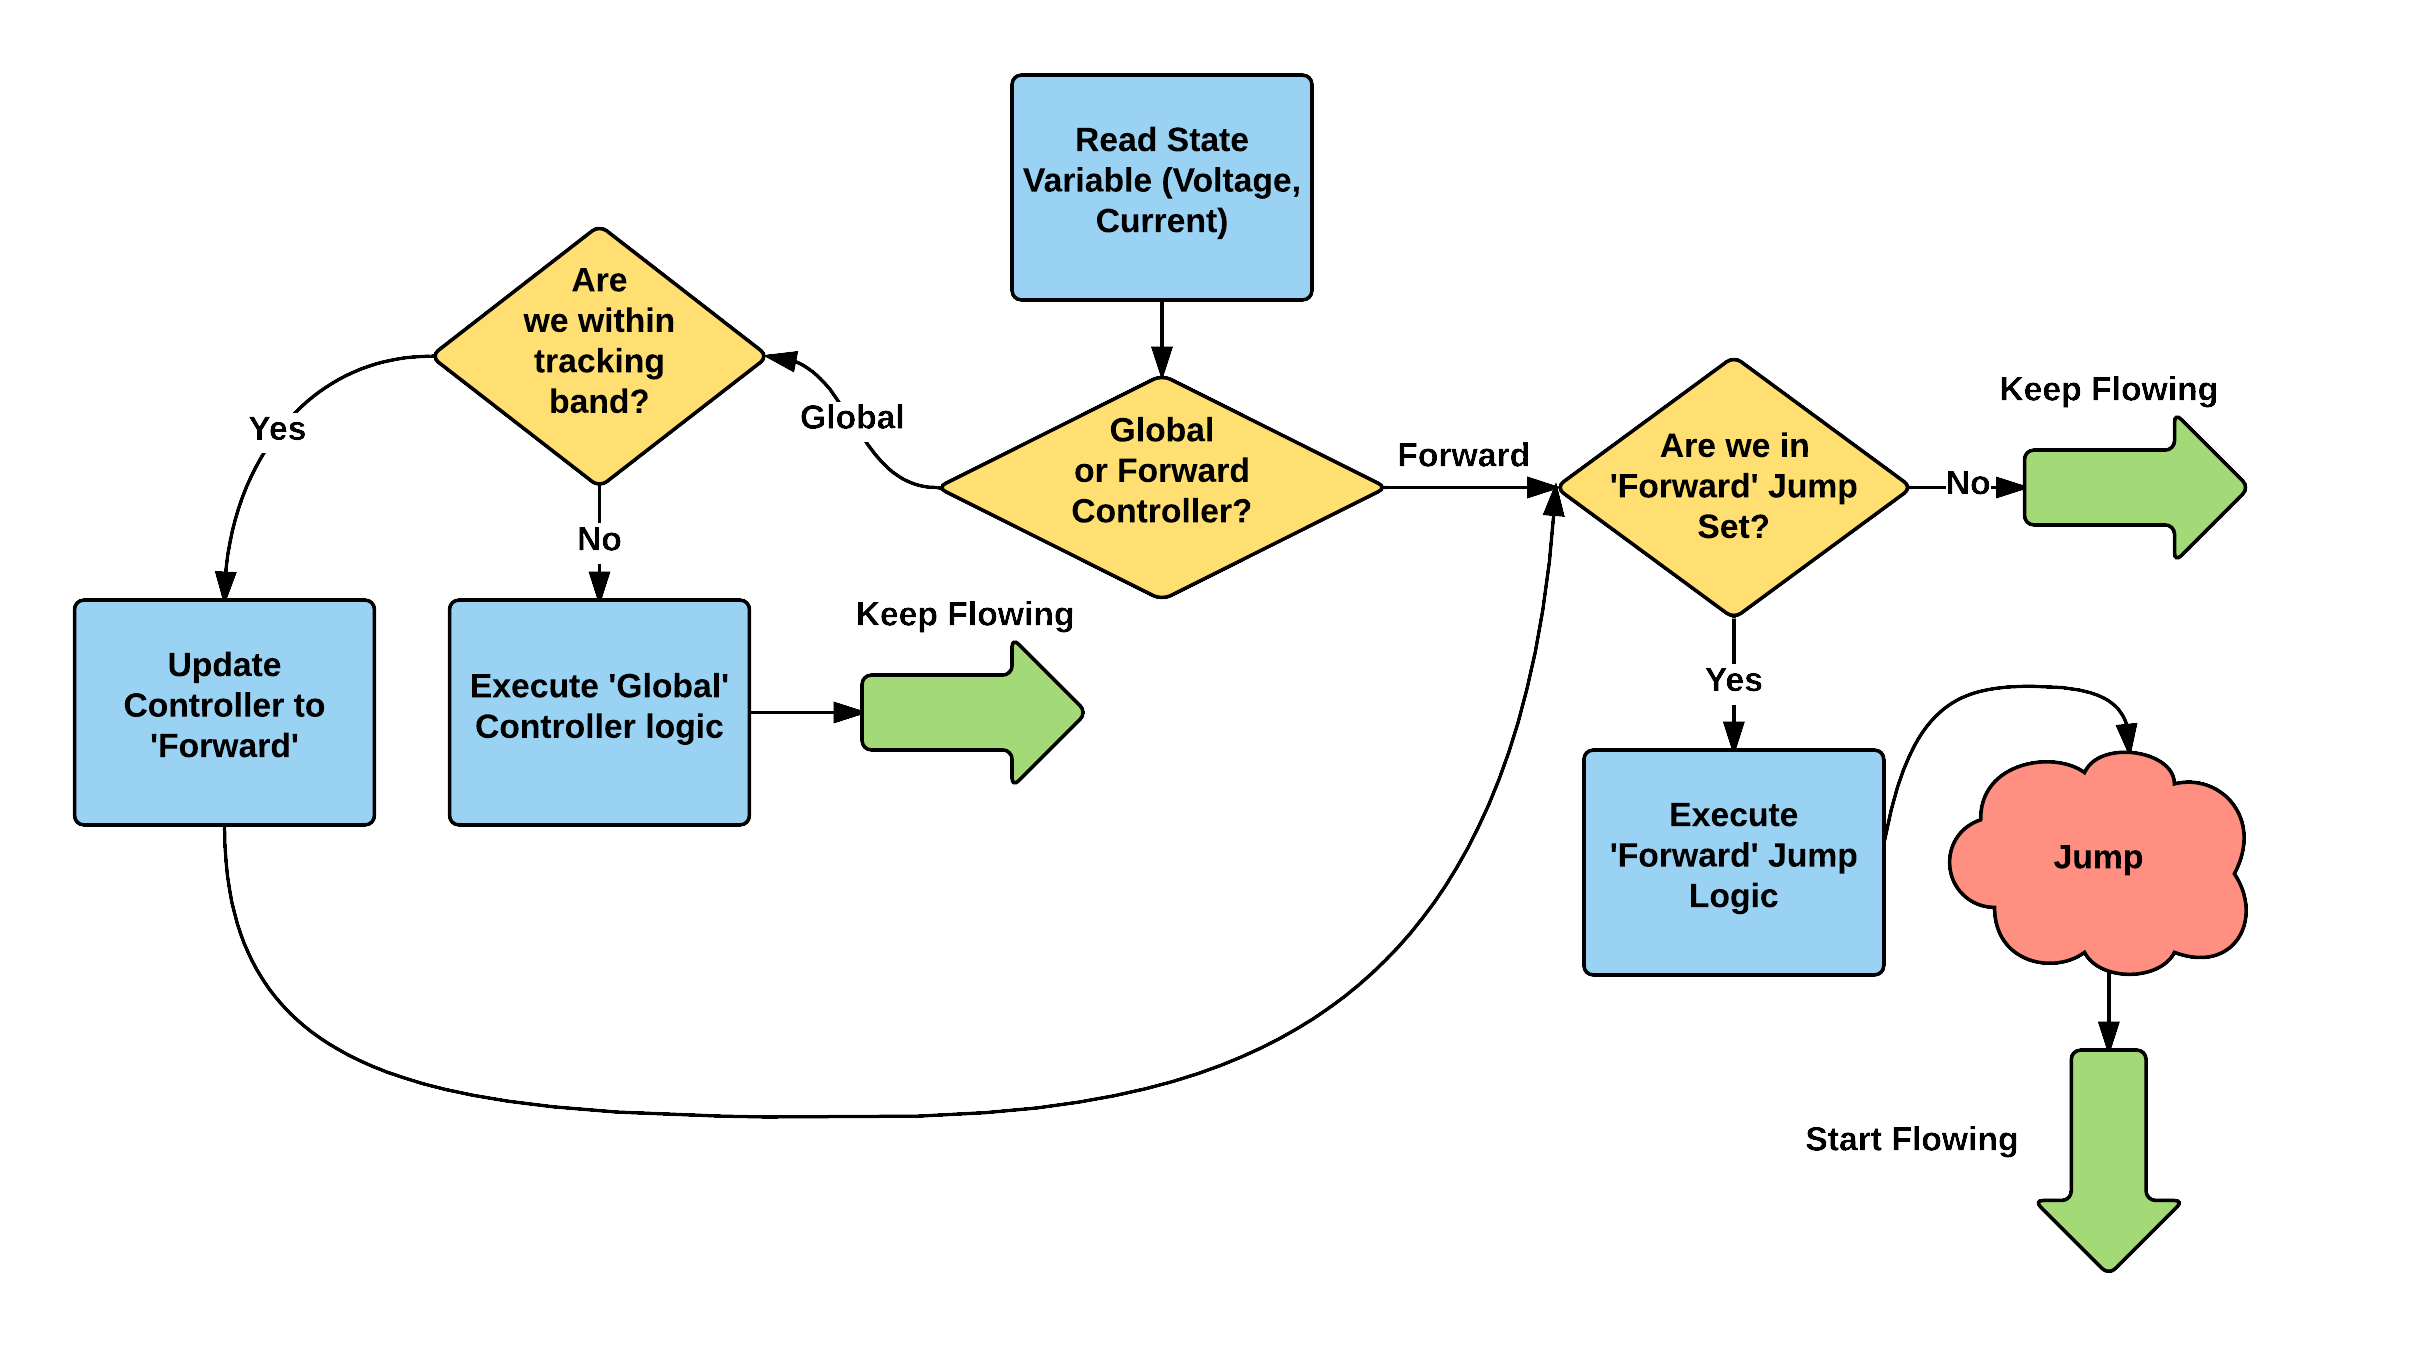
\includegraphics[width = 6 in]{hybridLogic}
\caption{Flow chart of the logic invloved with executing the `Hybrid Jump Logic' within the hybrid PWM inverter ISR}
\label{fast}
\end{center}
\end{figure}

The proper operation of the controller depends on it's interface with hardware; therefore, we will briefly cover the initialization of the PWM driver that we use to control the H-bridge. Adjacent PWM modules, namely PWM1 and PWM 2, are used to operate the half-bridge modules that make up the complete H-Bridge of our inverter. Each PWM module drives two PWM signals that are configured to be duals of one another - this prevent shoot-through in the H-bridge. These two signals are designated by PMWxA or PWMxB, where x is the number of the module, and A and B represent the two PWM signals of each module. In our implementation, PWMxA of each modules drives the low-side FET of each leg, while PWMxB drives the high side FET. 

In our hardware setup, we configure parameters like deadband, counting mode, period and phase synchronization for the adjacent PWM modules driving our H-bridge. The driver function itself - because we are operating the PWM in hybrid mode as simple $0$ or $100\%$ duty cycle - utilizes the fact that we can set the trip of the ePWM modules to a period greater or less than the timer can ever reach. In this way, we can operate the PWM modules essentially as GPIO pins that are either logic high or logic low without reconfiguring the hardware to treat these pins as GPIO. This functionality could potentially allow for `hot-swapping' between hybrid and traditional PWM operation, although we do not make use of such a functionality at this time. Secondarily, the use of PWM modules to produce $0$ and $100\%$ duty cycles allows for the use of control law accelerator (CLA) functionality in future revisions. 

The PWM driver function was written as follows:
\lstset{frame=tb,
  language=C,
  aboveskip=3mm,
  belowskip=3mm,
  showstringspaces=false,
  columns=flexible,
  basicstyle={\small\ttfamily},
  numbers=none,
  numberstyle=\tiny\color{gray},
  keywordstyle=\color{blue},
  commentstyle=\color{dkgreen},
  stringstyle=\color{mauve},
  breaklines=true,
  breakatwhitespace=true,
  tabsize=1
}
\begin{lstlisting}[label={lst:driver}]
#define PWMDRV_Hybrid(v)
	if ( v == VDC)
	{
		(*ePWM[n]).CMPA.half.CMPA	= TBPRD + 1;
		(*ePWM[n+1]).CMPA.half.CMPA	= 0;
	}
	else if (v == ZERO_VDC){
		(*ePWM[n]).CMPA.half.CMPA	= 0 ;
		(*ePWM[n+1]).CMPA.half.CMPA	= 0;
	}
	else if (v == NEG_VDC)
	{
		(*ePWM[n]).CMPA.half.CMPA	=  0;
		(*ePWM[n+1]).CMPA.half.CMPA	= TBPRD + 1;
	}
#endif
\end{lstlisting}

As shown in code example \ref{lst:driver}, putting a zero in the CMPA register of leg 2 (n+1) means that the high side fet on leg 2 is off, and the low side fet is on. Putting TBPRD+1 in the CMPA register of  leg 1 means that the low side fet is off, while the high side fet is on. 
The result is a current path from vdc through the load, and back down to ground (effectively $+V_{dc}$ at the load). Following an inverse logic, we can achieve $-V_{dc}$ at the load, as well as connecting the load to ground - effectively placing zero volts at the load - by driving both low side FETs.

After having properly configured the PWM modules for operation of an H-bridge, we can use the driver function to update the state of the H-Bridge with deadband for shoot-through protection. This driver function is called after the transition logic is executed, and the transition logic is executed only after the current state variable is constructed. Let's examine the update of the state variable on each iteration of the inverter ISR. 

\todo[inline]{update this as we calculate the phase and clarify logic!}
\begin{lstlisting}
	Vac_in = (long)((long)Vac_FB<<9)-Offset_Volt;	// shift to convert to Q21
	inv_ref_cur_inst = _IQ24mpy(inv_Iset, (((long) (InvSine)) << 9));

	inv_meas_cur_lleg1_inst=(((long) Ileg1_fb) <<12)-_IQ24(0.5);
	inv_meas_cur_lleg2_inst=(((long) Ileg2_fb) <<12)-_IQ24(0.5);

	inv_meas_cur_diff_inst = (inv_meas_cur_lleg1_inst - inv_meas_cur_lleg2_inst)<<1;

	inv_meas_vol_inst =((long)((long)Vac_FB<<12)-_IQ24(0.5))<<1;	// shift to convert to Q24


	updateState(&state, inv_ref_cur_inst, inv_meas_vol_inst, phase);
\end{lstlisting}
 
Once the state variable has been updated for the current iteration of the ISR, the state variable can be passed to the state machine operating the hybrid algorithm. This is done with the following code:

\todo[inline]{update this with the most recent code!}
\begin{lstlisting}
char HBridgeTransitionFunction(HBridge self, HBridgeEvent *e, StateVariable state)
{

    void   *funptr = self.super_.state__;

    il = state.current;
    vc = state.voltage;
    q = state.bridgeState;
    p = state.controller;
    
    /**
     * Determine which set the state variable belongs to: C or D
     */
    
    //Reset set membership status
    inC = false;   
    inD = false;

    Vz0 = (il/ALPHA)^2 + (vc/BETA)^2;

    /**
     * Supervisory Controller 
     * Determine if we need to switch controllers, depending on where the state variable is
     */
    if(state.controller == GLOBAL){
        if((Vz0 >= CIN) && (Vz0 <= COUT)){      // are we between the two tracking bands? -> select forward controller
            state.controller = FORWARD;
            //inD = true;
        }
    }
    else if(state.controller == FORWARD){
        if((Vz0 >= COUT) || (Vz0 <= CIN)){      // are we inside both, or outside both tracking bands? -> select global controller
            state.controller = GLOBAL;
        }
    }

    /** Forward Controller Check */
    if(state.controller == FORWARD)           
    {      
        if((Vz0 >= CIN) && (Vz0 <= COUT)){
            inC = true;
        }
        else{
            inC = false;            
        }

    }
    /** Global Controller Check */
    else if(state.controller == GLOBAL)   
    {     
        if((Vz0 <= CIN) && (Vz0 >= COUT)){
            inC = true;
        }
        else{
            inC = false;            
        }
    }

    /**
     * D:
     * Determining Jump Set membership
     */
    
    /**
     * Determine if we are in 'fast-swithcing regions' M1 or M2 so that we may respond accordingly
     */
    M1 = ((_IQabs(Vz0-cout) < ERROR) && ((state.current >= 0) && (state.current <= EPSILON)) && (state.voltage <= 0)) ? true:false;
    M2 = ((_IQabs(Vz0 - COUT) < ERROR) && ((state.current >= -EPSILON) && (state.current <= 0)) && (state.voltage >= 0)) ? true:false;

    /** Forward Controller Check */
    if(state.controller == FORWARD)           
    {      
        if(q != 0){
           if( (abs(Vz0-cin) <= ERR) && (il*q <= 0)){
               inD = 1;
           }
           else if( (abs(Vz0-cout) <= ERR) && (il*q >= 0)){
               inD = 1;
           }
       }
        else if (q == 0){
            if( (abs(Vz0-cin) <= ERR) && (q == 0)){
                inD = 1;
            }
        }
    }

    /** Global Controller CHeck */
    if(state.controller == GLOBAL){
        if((Vz0 >= cin) && (Vz0 <= cout)){
            inD = 1;
        }
    }

    /**
     * If we're in the jump set, determine which state transition to make
     * Else, dont waste clock cycles!
     */
    if(inD){

        /**
         * For the Hfw Controller
         */
        if(p == FORWARD){
            if(q != NEG_VDC){
                if( ((abs(Vz0-cout) <= ERR) && (il >= 0) && (~M1)) || (((abs(Vz0-cin) <= ERR)) && (il <= 0)) ){
                qplus = NEG_VDC;
                }
            }
            else if ( ((M1) && (abs(il - EPSILON) >= ERR) && (q == 1)) || ((M2) && (abs(il + EPSILON) >= ERR) && (q == -1)) ){
                    qplus = ZERO_VDC;
                }
            else if(q != VDC){
                if( ((abs(Vz0 - cout) <= ERR) && (il <= 0) && (~M2)) || (((abs(Vz0 - cin) <= ERR)) && (il >= 0)) ){
                    qplus = VDC;
                }
            }
            else{
                qplus = NO_EVENT;                
            }
        }

        /**
         * For the Hg Controller
         */
        else if(p == GLOBAL){
            if(Vz0 <= CIN){
                qplus = VDC;
            }
            else if(Vz0 >= COUT){
                qplus = ZERO_VDC;
            }
            else{
                qplus = NO_EVENT;
            }
        }
    }

    if(pplus != NO_EVENT){
        e->super_.signal = qplus;
        state.controller = qplus;       //q = qplus
    }

    return qplus;
}
\end{lstlisting}

The result of the C code above is identical to that in the Matlab iteration, save for the fact that it is superfluous to know whether or not we are in the flow set because they system is not solving any differential equations, but rather it is causing real hardware to execute in real-time.  Therefore, it is sufficient to determine whether or not we are in the jump set. Note that in the above code segment, there is no interface to hardware, only a change in the signal of the event 'e.' After the signal member of the event structure is set, this event gets dispatched to the current state (function), which performs the state transition. The current state of the machine is echoed in hardware via the hybrid PWM driver function. Thus, we have executed the full hybrid controller in C on our DSP. 

While PWM algorithms offer a relatively simple means for analyzing the switching waveform since we are modulating a carrier signal of known frequency. This is not quite the case for the hybrid algorithm where the switching occurs in response to where and when the state of the system leaves or enters the tracking band, how often we check it, and the with of the regions $M1$ and $M2$ shown in Figure \ref{jump}. An in-depth comparative analysis of the switching behavior of either algorithm is saved for Chapter \ref{Chapter5}.